%%%%%%%%%%%%%%%%%%%%%%%%%%%%%%%%%%%%%%%%%%%%%%%%%%%%%%%%%%%%%%%%%%%%%%%%%%%%%%%%%%%%
% Document data
%%%%%%%%%%%%%%%%%%%%%%%%%%%%%%%%%%%%%%%%%%%%%%%%%%%%%%%%%%%%%%%%%%%%%%%%%%%%%%%%%%%%
\documentclass[12pt]{article} %report allows for chapters
%%%%%%%%%%%%%%%%%%%%%%%%%%%%%%%%%%%%%%%%%%%%%%%%%%%%%%%%%%%%%%%%%%%%%%%%%%%%%%%%%%%%
\usepackage{preamble}
\newcommand{\vhat}{\boldsymbol{\hat{v}}}
\newcommand{\ehat}{\boldsymbol{\hat{e}}}
\newcommand{\Span}{\operatorname{Span}}

\begin{document}

\begin{center}
   \textsc{\large MATH 271, Homework 7, \emph{Solutions}}\\
   \textsc{Due November 1$^\textrm{st}$}
\end{center}
\vspace{.5cm}



\newpage
\begin{problem}
Consider the following vectors in the real plane $\R^2$. We let
\[
\vecu = 1\ehat_1 + 2\ehat_2 \qquad \textrm{and} \qquad \vecv = -3\ehat_1+ 3\ehat_2.
\]
\begin{enumerate}[(a)]
    \item What is the dimension of the vector space $\R^2$? Explain.
    \item Draw both $\vecu$ and $\vecv$ in the plane and label the origin.
    \item Draw the vector $\vecw = \vecu+\vecv$ in the plane.
    \item Draw the subspace spanned by $\vecu$.
    %\item Draw both $\vecu$ and $\vecv$ in the plane and label the origin.
    %\item Draw the vector $\vecw = \vecu+\vecv$ in the plane.
    %\item Find the area of the parallelogram generated by $\vecu$ and $\vecv$.
\end{enumerate}
\end{problem}
\begin{solution}
\begin{enumerate}[(a)]~
    %\item See the plane below.
    \item The dimension of $\R^2$ is 2. For example, we can take the set of vectors $\ehat_1$ and $\ehat_2$ and note that these vectors are linearly independent and span $\R^2$ and therefore are a basis for $\R^2$. Since two vectors constitute a basis, it must be the dimension is two. \emph{This set $\ehat_1$ and $\ehat_2$ is called the standard basis for $\R^2$.}
    \item Shown in the plot below.
    \item Here are $\zerovec$, $\vecu$, and $\vecv$ along with their sum $\vecu+\vecv$.
    \begin{center}
        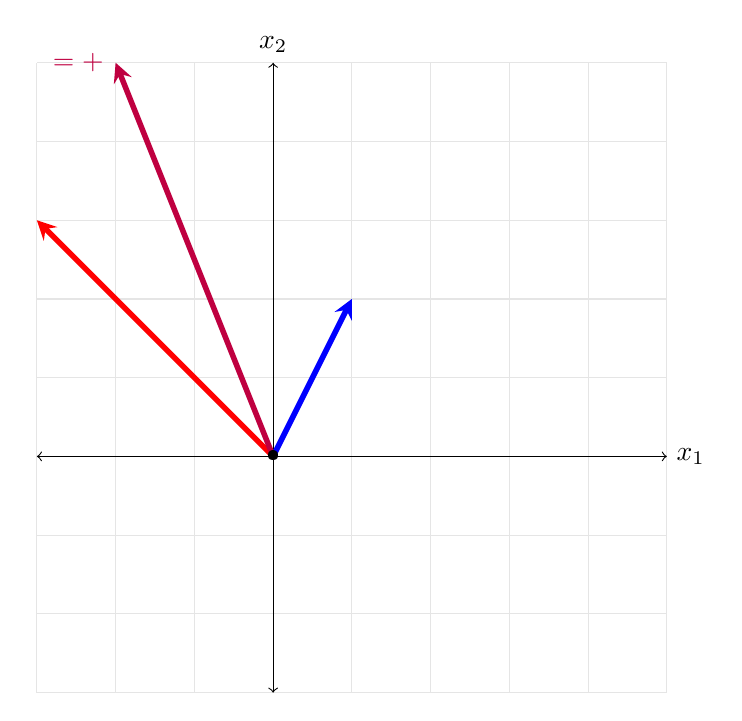
\begin{tikzpicture}
        \draw[thin,gray!20] (-3,-3) grid (5,5);
        \draw[<->] (-3,0)--(5,0) node[right]{$x_1$};
        \draw[<->] (0,-3)--(0,5) node[above]{$x_2$};

        \draw[line width=2pt,blue,-stealth](0,0)--(1,2) node[anchor=west] at (1,2){$\vecu$};
        \draw[line width=2pt, red, -stealth](0,0)--(-3,3) node[anchor=north] at (-3,3){$\vecv$};
        \draw[line width=2pt, purple, -stealth](0,0)--(-2,5) node[anchor=east] at (-2,5){$\vecw = \vecu+\vecv$};
        \node at (0,0){\textbullet};
        \node at (0,0)[right]{$\zerovec$};

        \end{tikzpicture}
        \end{center}

\item The subspace spanned by $\vecu$ is the set of all linear combinations of $\vecu$. Let us refer to this space as $U$ and, by definition this is all linear combinations of the vector $\vecu$
\[
U = \Span\{\vecu\} = \{ \alpha \vecu ~\vert~ \alpha \in \R\}.
\]
If you'd like, this can be written as
\[
U = \begin{pmatrix} \alpha \\ 2\alpha \end{pmatrix}, \quad \alpha \in \R,
\]
which is given by the following picture:
    \begin{center}
        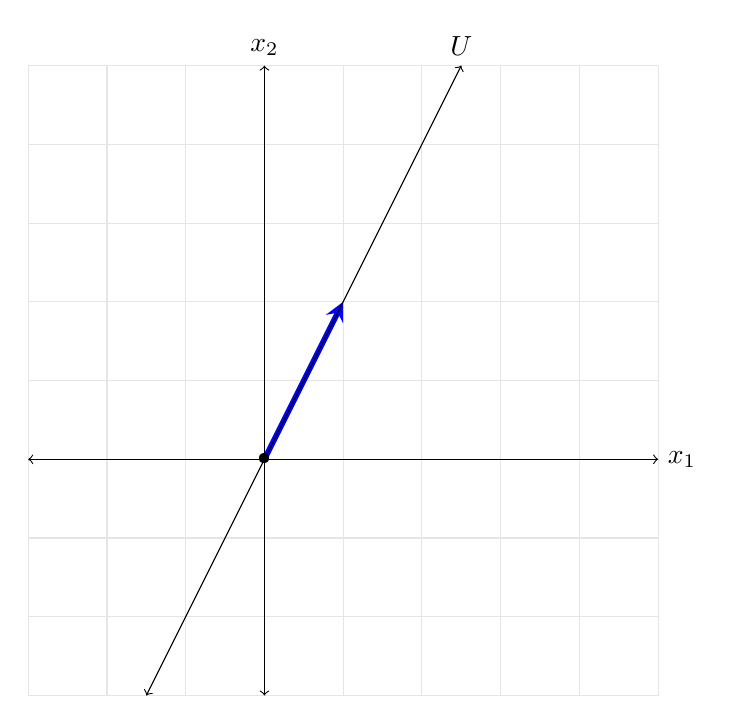
\begin{tikzpicture}
        \draw[thin,gray!20] (-3,-3) grid (5,5);
        \draw[<->] (-3,0)--(5,0) node[right]{$x_1$};
        \draw[<->] (0,-3)--(0,5) node[above]{$x_2$};

        \draw[line width=2pt,blue,-stealth](0,0)--(1,2) node[anchor=west] at (1,2){$\vecu$};
        \draw[<->] (-1.5,-3)--(2.5,5) node[above]{$U$};
        \node at (0,0){\textbullet};
        \node at (0,0)[right]{$\zerovec$};

        \end{tikzpicture}
        \end{center}
\end{enumerate}
\end{solution}

 %%%%%%%%%%%%%%%%%%%%%%%%%%%%%%%%%%%%%%%%%%%%%%%%%%%%%%%%%%%%%%%%%%%%%%%%%%%%%%%%%%%%%%%%%%%%
\newpage
\begin{problem}
Let a mass $m_1$ weighing $1kg.$ be placed at $\vecr_1=2\xhat -3 \yhat -\zhat$ and a mass $m_2$ of $2kg.$ be placed at $\vecr_2 = 4\yhat -2\zhat$.  Where must a mass $m_3$ of $3kg.$ be placed so that the center of mass is at the origin $\zerovec$?
\end{problem}
\begin{solution}
One can compute the center of mass $\boldsymbol{\vec{R}}_{CM}$ by
\[
\boldsymbol{\vec{R}}_{CM} = \frac{m_1\vecr_1 + m_2\vecr_2 + m_3 \vecr_3}{m_1 + m_2 + m_3}.
\]
Here, we know everything but $\vecr_3$.  Since we want the center of mass at the origin $\zerovec$, then
\begin{align*}
\zerovec &= \frac{1}{m_1+m_2 + m_3} \left( m_1 \vecr_1 + m_2 \vecr_2 + m_3 \vecr_3 \right)\\
\begin{pmatrix} 0 \\ 0 \\ 0\end{pmatrix}&= \frac{1}{6} \left( \begin{pmatrix} 2 \\ -3 \\ -1 \end{pmatrix} + 2 \begin{pmatrix} 0 \\ 4 \\ -2 \end{pmatrix} + 3 \begin{pmatrix} x \\ y \\ z \end{pmatrix}\right).
\end{align*}
What we have above is three equations and three unknowns. That is, one equation for the $\xhat$-component, one for the $\yhat$-component, and one for the $\zhat$-component. We have
\begin{align*}
    0 & = \frac{1}{6} (2 + 2\cdot 0 + 3x)\\
    0 & = \frac{1}{6} (-3 + 2\cdot 4 + 3y)\\
    0 & = \frac{1}{6} (-1 +2\cdot (-2) + 3z).
\end{align*}
Taking the first, we find
\begin{align*}
    0&= \frac{1}{3} +\frac{1}{2}x\\
    -\frac{1}{3}&= \frac{1}{2}x\\
    \implies~ x&= -\frac{2}{3}.
\end{align*}
Next,
\begin{align*}
    0&= -\frac{1}{2} +\frac{4}{3}+\frac{1}{2}y\\
    -\frac{5}{6}&= \frac{1}{2}y\\
    \implies~ y&= -\frac{5}{3}.
\end{align*}
Lastly, we have
\begin{align*}
    0&= -\frac{1}{6}-\frac{2}{3} +\frac{1}{2}z\\
    \frac{5}{6} &= \frac{1}{2}z\\
    \implies~ z&= \frac{5}{3}.
\end{align*}
Thus we have that $\vecr_3 = -\frac{2}{3} \xhat - \frac{5}{3}\yhat + \frac{5}{3}\zhat.$
\end{solution}

 %%%%%%%%%%%%%%%%%%%%%%%%%%%%%%%%%%%%%%%%%%%%%%%%%%%%%%%%%%%%%%%%%%%%%%%%%%%%%%%%%%%%%%%%%%%%
\newpage
\begin{problem}
Which of the following are linear transformations? For those that are not, which properties of linearity (the properties (i) and (ii) in our notes) fail? Show your work.
\begin{enumerate}[(a)]
    \item $T_a \colon \R \to \R$ given by $T_a(x)=\frac{1}{x}$.
    \item $T_b \colon \R^3 \to \R^2$ given by
    \[
    T_b \begin{pmatrix} x\\ y\\ z \end{pmatrix}
    = \begin{pmatrix} x\\ y \end{pmatrix}.
    \]
    \item $T_c \colon \R \to \R^3$ given by
    \[
    T_c(t)=\begin{pmatrix} t\\ t^2\\ t^3 \end{pmatrix}.
    \]
    \item $T_d \colon \R^2 \to \R^3$ given by
    \[
    T_d \begin{pmatrix} x\\ y \end{pmatrix}
    = \begin{pmatrix} x+y\\ x+y\\ x+y \end{pmatrix}.
    \]
\end{enumerate}
\end{problem}
\begin{solution}~
\begin{enumerate}[(a)]
    \item This transformation fails both properties.  For (i), take
    \[
    T_a(x+y) = \frac{1}{x+y} \neq \frac{1}{x}+\frac{1}{y} = T_a(x)+T_a(y).
    \]
    For (ii), take
    \[
    T_a(\alpha x) = \frac{1}{\alpha x} \neq \alpha \frac{1}{x} = \alpha T_a(x).
    \]
    \item This is a linear transformation.  To see (i) holds, take
    \begin{align*}
        T_b(\vecu +\vecv)&= T_b \left( \begin{pmatrix} u_x \\ u_y \\ u_z \end{pmatrix} + \begin{pmatrix} v_x \\ v_y \\ v_z \end{pmatrix} \right)\\
        &=T_b \begin{pmatrix} u_x + v_x \\ u_y + v_y \\ u_z + v_z \end{pmatrix}\\
        &= \begin{pmatrix} u_x + v_x \\ u_y + v_y \end{pmatrix}\\
        &= \begin{pmatrix} u_x \\ u_y \end{pmatrix} + \begin{pmatrix} v_x \\ v_y \end{pmatrix}\\
        &= T_b(\vecu) + T_b(\vecv).
    \end{align*}
    And for (ii), we take
    \begin{align*}
        T_b(\alpha \vecv) &= T_b \left( \alpha \begin{pmatrix} v_x \\ v_y \\ v_z \end{pmatrix}\right)\\
        &= T_b \begin{pmatrix} \alpha v_x \\ \alpha v_y \\ \alpha v_z \end{pmatrix}\\
        &= \begin{pmatrix} \alpha v_x \\ \alpha v_y \end{pmatrix}\\
        &= \alpha \begin{pmatrix} v_x \\ v_y \end{pmatrix}\\
        &= \alpha T_b(\vecv).
    \end{align*}
    \item This is not a linear transformation as both properties fail. Indeed, for (i) we take
    \begin{align*}
        T_c(\vecu +\vecv) &= T_c \left( \begin{pmatrix} u_x \\ u_y \\ u_z \end{pmatrix} + \begin{pmatrix} v_x \\ v_y \\ v_z \end{pmatrix} \right)\\
        &= T_c \begin{pmatrix} u_x + v_x \\ u_y + v_y \\ u_z + v_z \end{pmatrix}\\
        &= \begin{pmatrix} u_x + v_x \\ (u_y + v_y)^2 \\ (u_z + v_z)^3 \end{pmatrix},
    \end{align*}
    whereas
    \begin{align*}
    T_c (\vecu)+T_c(\vecv) &= T_c \begin{pmatrix} u_x \\ u_y \\ u_z \end{pmatrix} +T_c\begin{pmatrix} v_x \\ v_y \\ v_z \end{pmatrix}\\
    &= \begin{pmatrix} u_x \\ u_y^2 \\ u_z^3 \end{pmatrix} + \begin{pmatrix} v_x \\ v_y^2 \\ v_y^3 \end{pmatrix}\\
    &= \begin{pmatrix} u_x + v_x \\ u_y^2 + v_y^2 \\ u_z^3 + v_z^3 \end{pmatrix}.
    \end{align*}
    Note that $u_y^2+v_y^2\neq (u_y+v_y)^2$ and $u_z^3+v_z^3\neq (u_z+v_z)^3$.

    To see that (ii) does not hold, take
    \begin{align*}
        T_c(\alpha \vecv ) &= T_c\begin{pmatrix} \alpha v_x \\ \alpha v_y \\ \alpha v_z \end{pmatrix}\\
        &= \begin{pmatrix} \alpha v_x \\ \alpha^2 v_y^2 \\ \alpha^3 v_z^3\end{pmatrix},
    \end{align*}
    whereas
    \begin{align*}
        \alpha T_c(\vecv)&= \begin{pmatrix} \alpha v_x \\ \alpha v_y^2 \\ \alpha v_z^3\end{pmatrix}.
    \end{align*}
    These are clearly not equal for every scalar $\alpha$.
    \item This function is linear. For (i), we have
    \begin{align*}
        T_d(\vecu + \vecv) &= T_d \begin{pmatrix} u_x + v_x \\ u_y + v_y \end{pmatrix}\\
        &=\begin{pmatrix} (u_x+v_x)+(u_y+v_y) \\ (u_x+v_x)+(u_y+v_y) \\ (u_x+v_x) + (u_y +v_y) \end{pmatrix}\\
        &= \begin{pmatrix} u_x + u_y \\ u_x + u_y \\ u_x + u_y \end{pmatrix} + \begin{pmatrix} v_x + v_y \\ v_x + v_y \\ v_x + v_y \end{pmatrix}\\
        &= T(\vecu) + T(\vecv).
    \end{align*}
    And for (ii) we have
    \begin{align*}
        T_d(\alpha \vecv) &= T_d \begin{pmatrix} \alpha v_x \\ \alpha v_y \end{pmatrix}\\
        &= \begin{pmatrix} \alpha v_x + \alpha v_y \\ \alpha v_x + \alpha v_y \\ \alpha v_x + \alpha v_y \end{pmatrix}\\
        &= \alpha T_d(\vecv).
    \end{align*}
\end{enumerate}
\end{solution}

 %%%%%%%%%%%%%%%%%%%%%%%%%%%%%%%%%%%%%%%%%%%%%%%%%%%%%%%%%%%%%%%%%%%%%%%%%%%%%%%%%%%%%%%%%%%%
\newpage
\begin{problem}~
\begin{enumerate}[(a)]
    \item We can reflect an arbitrary vector in the plane by defining a function that reflects the basis vectors and extending the function with linearity. Let $R\colon \R^2 \to \R^2$ be a function be defined by
    \[
    R(\ehat_1) = -\ehat_1 \qquad \textrm{and} \qquad R(\ehat_2)=\ehat_2.
    \]
    Let $\vecv = v_1 \ehat_1 + v_2 \ehat_2$ and let
    \[
    R(\vecv) = v_1 R(\ehat_1) + v_2 R(\ehat_2).
    \]
    Show that $R$ reflects the vector $\vecu = 1\ehat_1 + 2\ehat_2$ about the $x_2$-axis and draw a picture.
    \item We can rotate a vector in the plane by first rotating the basis vectors $\ehat_1$ and $\ehat_2$. Define a linear function $J\colon \R^2 \to \R^2$ defined by
    \[
    J(\ehat_1)=\ehat_2 \qquad \textrm{and} \qquad J(\ehat_2)=-\ehat_1.
    \]
    \noindent Show that $J$ rotates $\vecu$ by $\pi/2$ in the counterclockwise direction and draw a picture.
\end{enumerate}
\end{problem}
\begin{solution}~
\begin{enumerate}[(a)]
    \item So, we can take the vector $\vecu$ and then we have
    \[
    R(\vecu)=1R(\ehat_1)+2R(\ehat_2) = -\ehat_1 +2\ehat_2.
    \]
    So we can plot both $\vecu$ and $R(\vecu)$ in the plane:
        \begin{center}
        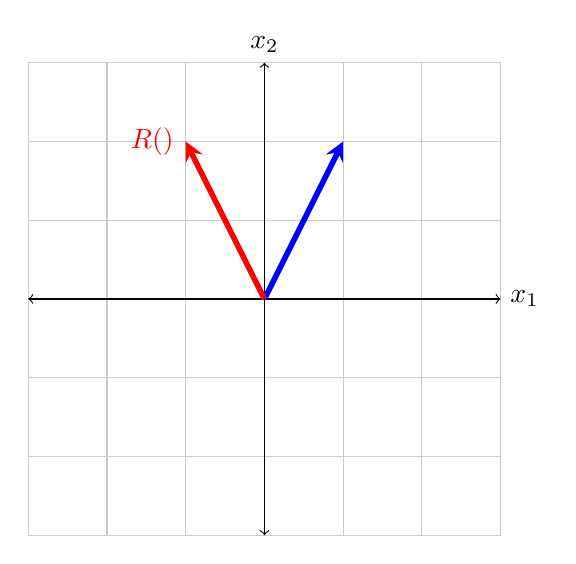
\begin{tikzpicture}
        \draw[thin,gray!40] (-3,-3) grid (3,3);
        \draw[<->] (-3,0)--(3,0) node[right]{$x_1$};
        \draw[<->] (0,-3)--(0,3) node[above]{$x_2$};
        \draw[line width=2pt,blue,-stealth](0,0)--(1,2) node[anchor=west] at (1,2){$\vecu$};
        \draw[line width=2pt, red, -stealth](0,0)--(-1,2) node[anchor=east] at (-1,2){$R(\vecu)$};
        \end{tikzpicture}
        \end{center}
        We can see that this is definitely the reflection of the vector $\vecu$ across the $y$-axis.
    \item We can now do this for the function $T$ to get
    \[
    J(\vecu) = J(\ehat_1)+2J(\ehat_2)=\ehat_2 -2\ehat_1.
    \]
    Then we can plot both $\vecu$ and $J(\vecu)$ in the plane:
        \begin{center}
        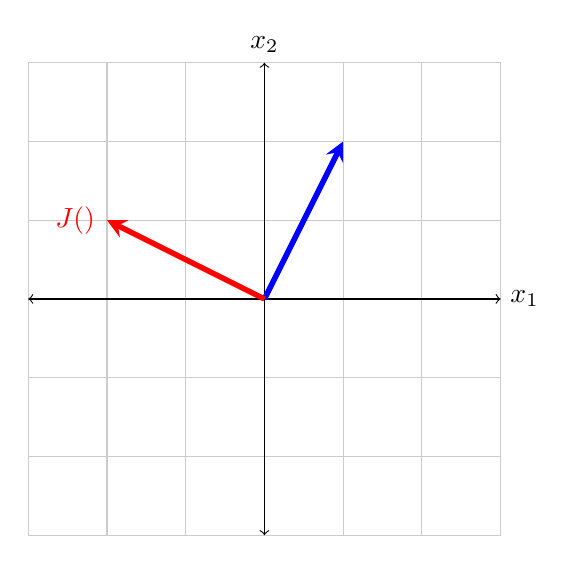
\begin{tikzpicture}
        \draw[thin,gray!40] (-3,-3) grid (3,3);
        \draw[<->] (-3,0)--(3,0) node[right]{$x_1$};
        \draw[<->] (0,-3)--(0,3) node[above]{$x_2$};
        \draw[line width=2pt,blue,-stealth](0,0)--(1,2) node[anchor=west] at (1,2){$\vecu$};
        \draw[line width=2pt, red, -stealth](0,0)--(-2,1) node[anchor=east] at (-2,1){$J(\vecu)$};
        \end{tikzpicture}
        \end{center}
        We can see that this is definitely the rotation  of the vector $\vecu$ an angle of $\pi/2$ in the counter-clockwise direction.
\end{enumerate}
\end{solution}

%\newpage
%\begin{problem}
%Consider the following vectors in space $\R^3$
%\[
%\vecu = 1\xhat + 2\yhat + 3\zhat \qquad \textrm{and} \qquad \vecv = -2\xhat +1\yhat -2\zhat.
%\]
%\begin{enumerate}[(a)]
%    \item Compute the dot product $\vecu\cdot \vecv$.
%    \item Compute the cross product $\vecu \times \vecv$.
%    \item Compute the lengths $\|\vecu\|$ and $\|\vecv\|$ using the dot product.
%    \item Compute the angle between vectors $\vecu$ and $\vecv$.
%    \item Compute the projection of $\vecu$ in the direction of $\vecv$.
%\end{enumerate}
%\end{problem}
%\begin{solution}~
%\begin{enumerate}[(a)]
%    \item We have that
%    \begin{align*}
%        \vecu \cdot \vecv &= 1\cdot (-2) + 2 \cdot 1 + 3 \cdot (-3)\\
%        &= -6.
%    \end{align*}
%    \item Here, feel free to use a formula for a cross product instead of writing it all out.  We will find that
%    \begin{align*}
%        \vecu \times \vecv &= -7\xhat -4\yhat +5\zhat.
%    \end{align*}
%    \item We compute the lengths using the dot product by
%    \[
%        \|\vecu\| = \sqrt{\vecu \cdot \vecu} = \sqrt{1^2+2^2+3^2} = \sqrt{14}.
%    \]
%    Likewise
%    \[
%        \|\vecv\| = \sqrt{\vecv \cdot \vecv} = \sqrt{(-2)^2 + 1^2 (-2)^2} = \sqrt{9} = 3.
%    \]
%    \item We can find the angle $\theta$ between $\vecu$ and $\vecv$ with the information we already have.  Indeed, recall the formula
%    \[
%        \vecu \cdot \vecv = \|\vecu \| \|\vecv\| \cos \theta.
%    \]
%    In the previous parts, we have computed $\vecu \cdot \vecv = -6$, $\|\vecu\|=\sqrt{14}$, and $\|\vecv\|=3$ so we now just have the following
%    \[
%        -6 = 3\sqrt{14} \cos \theta.
%    \]
%    Thus,
%    \[
%        \theta = \arccos\left(\frac{-6}{3\sqrt{14}}\right) \approx 2.1347 ~\textrm{radians}.
%    \]
%    One could also use the fact that $\|\vecu \times \vecv\| = \|\vecu\| \|\vecv\| \sin \theta$ since we had already compute the cross product earlier.
%    \item The projection of $\vecu$ in the direction of $\vecv$ is simply asking for how much of the vector $\vecu$ is in the direction of $\vecv$.  One can arrive at this purely through trigonometry, but we have the dot product at our disposal.  The normalized vector $\vhat$ points in the direction of $\vecv$ with length 1 and
%    \[
%        \vhat = \frac{1}{\|\vecv\|} \vecv = \frac{1}{3} \vecv.
%    \]
%    Then, the projection can be computed by
%    \[
%        \vecu \cdot \vhat = \frac{1}{3} \vecu \cdot \vecv = -2.
%    \]
%    One should attempt to recover this notion by doing some trigonometry.
%\end{enumerate}
%\end{solution}

\begin{problem}
Let $S$ be the set of general solutions to the following second order homogeneous linear differential equation
\[
x''+f(t)x'+g(t)x=0.
\]
Show that this set $S$ is a vector space over the field of complex numbers.
\end{problem}
\begin{solution}
    We can remember these requirements via the acronym CANI ADDU.  So we have for the vector addition properties
    \begin{itemize}
        \item Commutivity: If we have two solutions $x(t)$ and $y(t)$ in the set $S$, then we know
        \[
        x(t)+y(t)=y(t)+x(t)
        \]
        is satisfied.
        \item Associativity: If we have three solutions $x(t),y(t),z(t)\in S$, then we know
        \[
        (x(t)+y(t))+z(t)=x(t) + (y(t)+z(t))
        \]
        is satisfied.
        \item Neutral Element: We have that there exists the zero function $0\in S$ such that
        \[
        0+x(t)=x(t).
        \]
        This is true since $0$ is a solution to the ODE.
        \item Inverses: Given an $x(t)\in S$, we have the function $-x(t)\in S$ such that
        \[
        x(t)+(-x(t))=0.
        \]
        This is true since $x$ is a solution implies that $-x$ also is.
    \end{itemize}
    Then we have the scalar multiplication properties
    \begin{itemize}
        \item Associativity: If we have $\alpha,\beta \in \C$ and $x(t)\in S$ then we have
        \[
        \alpha (\beta x(t)) = (\alpha \beta)x(t)
        \]
        holds.
        \item Distribution: Given $\alpha,\beta \in \C$ and $x(t)\in S$ we have
        \[
        (\alpha +\beta)x(t) = \alpha x(t) + \beta x(t)
        \]
        holds.
        \item Distribution: Given $\alpha\in \C$ and $x(t),y(t)\in S$, we have
        \[
        \alpha(x(t)+y(t))=\alpha x(t) + \alpha y(t)
        \]
        holds.
        \item Unit element: We have $1\in \C$ satisfies that for any $x(t)\in S$ that
        \[
        1 x(t) = x(t).
        \]
    \end{itemize}

    \begin{remark}
        Not all vector spaces will have such obvious neutral elements, $\zerovec$. Likewise, not all fields will have an obvious unit element $1$.  This is why we must be a bit careful at times. Take for example the vector space whose field elements are \textbf{TRUE} and \textbf{FALSE} values.
    \end{remark}
    Now, the biggest requirement for a vector space is that linear combinations of vectors actually produce another vector. This is quite obvious in the plane $\R^2$ for example, but here, it is not necessarily obvious. To see this, take $\alpha,\beta \in \C$ and $x(t),y(t)\in S$ and we consider the linear combination
    \[
    z(t) = \alpha x(t) + \beta y(t).
    \]
    We then wish to show that this linear combination (or superposition) is a solution as well. So we plug in $z(t)$ into our equation as follows
    \begin{align*}
        z''(t)+f(t)z'(t)+g(t)z(t)&= (\alpha x''(t) + \beta y''(t))+f(t)(\alpha x'(t) + \beta y'(t))+g(t)(\alpha x(t)+\beta y(t))\\
        &= \alpha \left[x''(t)+f(t)x'(t)+g(t)x(t)\right] + \beta \left[ y''(t)+f(t)y'(t)+g(t)y(t)\right]\\
        &=0,
    \end{align*}
    since we knew that $x(t)$ and $y(t)$ themselves are solutions. Thus, $z(t)$ is as well and now we have that $S$ is a vector space. It is worth noting that we have shown this result in previous work.
\end{solution}

\newpage
\begin{problem}
Let $P_3(\mathbb{C})$ be the vector space of polynomials of degree at most 3 with coefficients in $\C$ with variable $x$. For example,
\[
f(x)= x^2+1 \in P_3(\mathbb{C}).
\]
\begin{enumerate}[(a)]
    \item Write down a basis for $P_3(\mathbb{C})$.
    \item What is the dimension of the vector space $P_3(\mathbb{C})$.
    \item Let $\frac{d}{dx} \colon P_3(\mathbb{C}) \to P_3(\mathbb{C})$. Argue that $\frac{d}{dx}$ is a linear transformation.
    \item What is the kernel (nullspace) of $\frac{d}{dx}$? What is the image (range) of $\frac{d}{dx}$?
\end{enumerate}
\end{problem}
\begin{solution}~
\begin{enumerate}[(a)]
    \item A basis for a space is a linearly independent set of vectors that spans the space. First, the most general polynomial of degree at most 3 with complex coefficients assumes the form
    \[
        p(x) = a_0 + a_1 x + a_2 x^2 + a_3 x^3
    \]
    where $a_j \in \C$ for $j=0,1,2,3$. Here, we are treating $x$ as a variable and we are not allowed to pick specific values for it -- we must leave it as is. We should also notice that specifying these polynomials in $P_3(\C)$ requires 4 coefficients -- one for $1$ ($a_0$), one for $x$ ($a_1$), one for $x^2$ ($a_2$), and finally one for $x^3$ ($a_3$). Let's take the set
    \[
    B=\{1, x,x^2,x^3\}
    \]
    and see if this suffices as a basis.
    \begin{enumerate}[i.]
        \item (Spaning set) First we show this set spans $P_3(\C)$. We have the arbitrary element $p(x)$, and a linear combination of our set looks like
        \[
        \alpha_0 1 + \alpha_1 x + \alpha_2 x^2 + \alpha_3 x^3.
        \]
        Setting this equal to $p(x)$ we notice that $\alpha_j = a_j$. So our set $B$ spans $P_3(\C)$.
        \item (Linearly independent) To see $B$ is linearly independent, suppose that
        \[
        \alpha_0 1 + \alpha_1 x + \alpha_2 x^2 + \alpha_3 x^3 = 0.
        \]
        Then, it must be that all $\alpha_j=0$ for $j=0,1,2,3$ and therefore this set is linearly independent.
    \end{enumerate}
    By the two points above, we have shown $B$ is a basis.

    \begin{remark}
    There are infinitely many other bases for $P_3(\C)$, but this one is \emph{standard} in a sense. Other bases may be nicer, for example, the legendre polynomials are a basis as well. These are,
    \[
     \left\{f_0 = \sqrt{\frac{1}{2}}, ~ f_1 = \sqrt{\frac{3}{2}}x, ~ f_2 = \sqrt{\frac{5}{8}} (1-3x^2),~ f_3=\sqrt{\frac{63}{8}}\left(x-\frac{5x^3}{3}\right) \right\}
    \]
    I'd claim this basis is nicer in certain circumstances. For example, we have shown it is \emph{orthogonal} and we also know they are in some sense solutions to a Schr\"odinger equation (they are \emph{eigenfunctions}).
    \end{remark}

    \item By (a), we have a basis of length 4, therefore the dimension is 4.

    \item Let $p(x), q(x) \in P_3(\C)$ then
    \begin{align*}
        \frac{d}{dx}(\alpha p+\beta q) &= \frac{d}{dx}(\alpha p) + \frac{d}{dx}(\beta q) && \textrm{by the sum rule}\\
        &= \alpha \frac{d}{dx}p + \beta \frac{d}{dx}q && \textrm{by the constant multiple rule},
    \end{align*}
    which shows $\frac{d}{dx}$ is linear. We can see that linearity is nothing but a combination of a sum and constant multiple rule.
    \item Applying $\frac{d}{dx}$ to $p(x)$ we have
    \begin{align*}
        \frac{d}{dx} p(x) &=\frac{d}{dx}( a_0 + a_1 x + a_2 x^2 + a_3 x^3)\\
        &= a_1 + 2a_2x + 3 a_3x^2.
    \end{align*}
    The above shows that $a_0$ was in the kernel of $\frac{d}{dx}$, so we can put
    \[
    \ker\left(\frac{d}{dx}\right) = \Span\{1\}.
    \]
    This is nothing but the fact you already know which states that derivatives of constants are zero. We also can see that after applying the derivative we end up with an arbitrary polynomial of degree at most 2. Therefore, we have
    \[
    \mathrm{im}\left( \frac{d}{dx}\right) = \Span \{1,x,x^2\}.
    \]
\end{enumerate}
\end{solution}

\end{document}